\section{Analysis of Depth Images} \label{sec:static_evaluation}
For a better understanding of the dynamic, the static behavior is analyzed in this section. The variance is the main dimension that will be investigated for that purpose. The static analysis is a measure for the noise floor. The variance should be as small as possible for a precise and accurate investigation of the dynamic investigation. It behaves as a disturbing dynamic that needs to be distinguished from the real dynamic. The analysis of absolute depth errors is not possible, since this requires a very precise experiment set-up. The positions must be adjusted over the complete range of $8~m$ in the resolution of the camera of $1~mm$. For a smaller range, this could be done on a lathe in the future. The following approaches shall give some rough estimations on the static behaviors. 

\subsection{Variance Depending on the Distance}   
The function of the variance $\sigma^2$ over different distances gives the fluctuation of a measurement in itself. As a consequence, the precision can be judged over the distance. Microsoft delivers its own measurement data of the standard derivation depending on the distance \cite{payne20147}. A direct comparison is not possible. The area that is kept fixed for the analysis is unknown. A translation between the variance $\sigma^2$ and the standard deviation $\sigma$ is possible by the following equation:

\begin{equation}
\sigma = \sqrt{\sigma^2}
\end{equation}

A white screen for overhead projectors with a very high diffuse reflectance of about $80\%$ has been captured over 3 seconds for the estimation of the variance. The investigated area is a 4x4 pixel window in the middle of the complete image. The area that is used for the dynamic investigations corresponds to this window. Therefore, the regions of the highest variance in the corners do not lie in the area. At the longest distance, the investigated area must still be completely on the screen. Afterwards, the mean variance of all pixels 16 is calculated in a time span of 3 seconds. The analysis has been done with the raw and TVD filtered data. As parameters for the filtering 20 iterations and $\lambda =1$ are used. The variance versus the distance is plotted additionally even if the measurement setup like the window size or the reflectivity is unknown \cite{payne20147}. 


\begin{figure}[!h]
	\centering
	\includegraphics[width=0.8\textwidth]{Bilder/Var_vs_distance_MS.png}
	\caption{Variance vs. distance Microsoft data, raw and TVD after 3 Seconds}
	\label{fig:Variance_TVDvsRAW}
\end{figure}

The comparison between the raw and filtered data in figure \ref{fig:Variance_TVDvsRAW} shows a significant reduction in the variance over the complete distance with TVD. The raw data has a quadratic trend. This results out of the quadratic decrease of the light intensity versus the distance to the camera. The light propagates on sphere area into the room as shown in equation \ref{eq:solid_angles}. The noise increases and the signal decreases with higher distances that correspond to a lower SNR. 

\subsection{Variance Depending on Geometries and Surfaces}
A simple way to investigate the variance difference between high reflecting white and low reflecting black surfaces is possible on a checkerboard. Squares of the same size on a flat surface are easy to distinguish with different reflectivity properties even if they lie on the same surface. This is also a common approach to calibrate the distortion of a standard camera objective. Figure \ref{fig:checkerboard} illustrates the change of the variance between the black and white areas in a one meter distance after a recording time of $3~s$. The black fields feature a higher variance than the white ones. The sticker material of the checkerboard has spread reflection characteristics. Therefore in the middle of the image more light is reflected backwards into to the sensor than on the outer areas. The variance in the middle is reduced. More light is reflected backwards. A calibration of the Kinect 2 is not necessary since the focal lens is fixed and the correction of the distortion is done in the image processing of the camera. 
The reflection characteristics on various material does not always behave in the same way as for visible light. This is shown on some random objects measured in there variance for a rough estimation between different surfaces. In figure \ref{fig:Material_Investigation}, a collection of geometries and surfaces are investigated. Except for the black flat plastic with a thick layer of clear paint and the polished aluminum pipe, all material probes show a low variance. The black plastic absorbs and spectral reflects most of the IR light and the pipe scatters the light in a spectral way to all sides. Only the middle part of the pipe parallel to the image plane is of low variance. More light is reflected backwards. Even if the heck spoiler and the copper sheet are spectral reflecting for visible light, this is not the case in the IR spectrum.\\ 

Flying pixels cause a high variance at the boarder of all objects. To distinguish small changes in the color space, larger variance values than $140~mm$ and distances behind the objects are set to zero. The influence of the angle to a plane surface has not been investigated. The change of variance on different geometries and surfaces should be part of further investigations. 

\begin{figure}[!h]
	\centering
	\includegraphics[width=0.77\textwidth]{Bilder/checkerboard.png}
	\caption{Variance on a checkerboard in $1~m$ distance}
	\label{fig:checkerboard}
\end{figure}

\begin{figure}[!h]
	\centering
	\includegraphics[width=0.77\textwidth]{Bilder/Material_Investigation.png}
	\caption{Variance on various geometries and surfaces}
	\label{fig:Material_Investigation}
\end{figure}

\subsection{Influence of Background Lighting on Static Measurements} \label{chap:static_Lighting}
The variance of the static bass membrane plays an impotent role for further dynamic analysis. A reduction in the noise characteristic is done with 5 white matt paper stickers attached to the membrane. This gives a clear sharp boarder to the original black surface. 2000 W of halogen light are pointed on the membrane to disturb the measurement from the position of the camera by a second IR light source. This data is compared with a recording in absolute darkness. The position and $1.4~m$ distance of the camera to the membrane are unchanged. The distribution of variances is illustrated in figure \ref{fig:membrane_static_dark} for the dark and in figure \ref{fig:membrane_static_halogen} under halogen lighting. The depth data of the background behind the membrane is set to zero. The light impact is remarkable on the black cone surface. The white paper is influenced much less by the IR lighting. The reason for that is the low SNR on the black cone. The IR light of the ToF measurement is strongly absorbed and scattered on this surfaces. With the IR impact of the halogen lighting, the noise is additionally increased to values higher than $500~mm$. This is caused by a spread spectral reflection, which directs a high amount of IR halogen light directly into the camera. The RGB image of the Kinect in figure \ref{fig:KinectScreenshot-Color-10-58-52} shows the same saturation caused by the spread reflection.

\begin{figure}[!h]
\subfigure[Variance on the static membrane in a dark room]{\includegraphics[width=0.5\textwidth]{Bilder/membrane_static_dark}\label{fig:membrane_static_dark}}\hfill
\subfigure[Variance on the static membrane and $2~kW$ halogen]{\includegraphics[width=0.5\textwidth]{Bilder/membrane_static_halogen.png}\label{fig:membrane_static_halogen}}
\centering
\caption{Influence of halogen lighting on the variance}
\end{figure}
 
\section{Evaluation of Membrane Dynamic} 
\subsection{Physical Model of Membrane Oscillation and Observation} \label{sec:bias_membrane}
This section delivers a physical model for the vibration of a subwoofer membrane in the investigated low frequency area $f_{ref} \leq 10~Hz$. Due to the low frequency excitation, every point moves with the same speed $\vec{v}(t)$ and the same phase into the normal direction $\vec{n}$ of the middle flat surface.  The measurement of the vibration under a bias angle is characterized by the angle between the optical axis and the surface normal, called viewing angle $\alpha$. Since LDV measures only the speed into the direction of the optical axis, the amplitude $A_{LDV}$ is reduced under higher angles to the surface normal. Figure \ref{fig:membrane_geometry} illustrates the basic geometries of the membrane observation. The viewing angle $\alpha$ is defined between the surface normal $\vec{n}$ and the optical axis turning into the negative mathematical direction. In contrast to that, the ToF amplitude $A_{ToF}$ is increased by the bias observation since the investigated pixels are moving sideways and ToF delivers the absolute distance and not a relative speed like LDV. With a cone angle $\beta$, the oblique areas delivers different normal surface angles and therefore $\alpha$ is changed. This physical model shows the relationship between the viewing angle $\alpha$ and the resulting amplitude of $A_{LDV}$ and $A_{ToF}$ represented by equation \ref{eq:tof_amplitude} and \ref{eq:ldv_amplitude}. This model assumes that the ToF camera has an infinite numbers of pixel. In practice this is not fulfilled. One pixel will therefore cover multiple distances under high angles. On the upper and lower surfaces the angle $\alpha_{l,u}$ depends on the oblique position of the cone surface and the angle $\beta$ to the middle surface. The coordinate system of the membrane is represented by the index (m) and has the same orientation as the scene plane coordinate system that is given by the depth images.  
  
\begin{equation}
A_{ToF} = A_m (\cos \alpha +1)
\label{eq:tof_amplitude}
\end{equation}

\begin{equation}
A_{LDV} = A_m \cdot \sin \alpha 
\label{eq:ldv_amplitude}
\end{equation}
 
\begin{equation}
\alpha_{l,u} = \alpha \pm \beta
\label{eq:alu_angle}
\end{equation}
\newpage

\begin{figure}[!h]
	\centering
	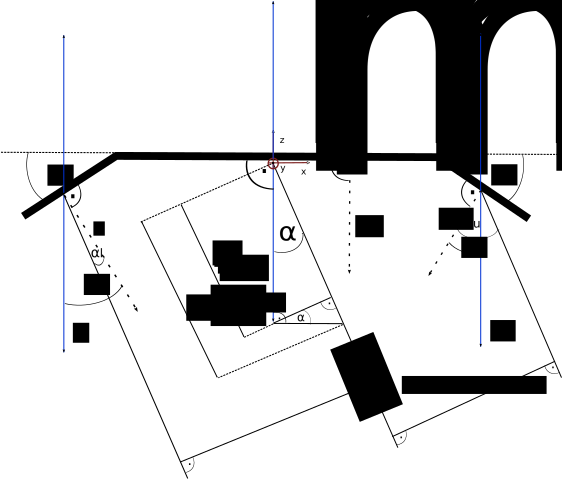
\includegraphics[width=0.8\textwidth]{Bilder/Geoemtry_membrane_amplitude.pdf}
	\caption{Geometry of bias membrane observation}
	\label{fig:membrane_geometry}
\end{figure} 

\bigskip
\begin{figure}[!h]
	\centering
	\includegraphics[width=0.9\textwidth]{Bilder/displacement_timedomain_membrane.png}
	\caption{Displacement of the membrane measured on the middle surface with a Laser Dopper Vibrometer under $\alpha = 0^\circ$}
	\label{fig:displacement_timedomain_membrane}
\end{figure} 

\newpage


\subsection{Scientific Problem} 
The dynamic behavior of a membrane is the test body for a detailed analysis of the ToF principle for dynamic measurement of surface vibrations. The membrane is excited and acquired under variable conditions to investigate multiple scenarios. A bass tube is plugged to a waveform generator, creating a defined vibration that is recovered from multiple ToF 3D scans. This data is compared with a Laser Doppler Vibrometer (LDV) as a reference. LDV delivers the accurate data of a single point on the membrane, whereas ToF measures the complete surface movement. Multiple questions will arise from that: One is the precision and accuracy distribution in frequency and amplitude over the membrane under different conditions. Which part cannot be investigated and which area is overlaid by noise? The influence of angle, distance, frequency and amplitude is questioned. How is the measurement influenced by an additional IR light source that emits in the same spectrum as the ToF laser diodes? Another questions is the influence of static filter method for the dynamic investigation. Is a reduction of the noise possible without an impact on the actual dynamic? Is the complete signal-to-noise-ratio influenced by the filtering? Can overtones like the first or second harmonic still be derived from the ToF data? How does ToF behave in a continuous change in frequency and amplitude? ToF allows the investigation of the complete field of view. How can the dynamic of a surface be illustrated? The following section tries to investigate all these questions in detail. The membrane movement should deliver an ideal test body, because it vibrates in only one direction at a stable frequency and amplitude. The vibration is controllable in frequency and amplitude. This approach could later be useful for the calibration of ToF for vibrations measurements with a scientific camera and under more controlled conditions. The experimental setup shall deliver first steps into this direction, showing the performance of ToF and, how the data can be processed in Matlab.   

\subsection{Hypothesis}  
With the depth resolution of $1~mm$ and a variance lower than $1.2~mm$ up to a distance of $2~m$, the system should be capable to distinguish changes of amplitude in the magnitude of the $1~mm$ depth resolution. Except for the corner of the images, a dynamic investigation in the whole field of view should be possible for distances blow $2.5~m$, because the variance in this distance is below or in the region of the depth resolution. Processed by a Fast-Fourier Transform, a vibration with a amplitude higher than $1~mm$ should always return the strongest peak in the frequency spectrum. With a sampling rate of $30~fps$ and an maximum vibration frequency of $10~Hz$, the limits of the Nyquist-Shannon theorem for dynamic measurements are satisfied. A precise determination in frequency should be possible on all areas of the membrane. An oversampling factor of 5 should be enough for the reconstruction of the wave form and amplitude. Therefore, every sinus period is sensed by 10 samples. Consequently, a precise reconstruction of a $3~Hz$ should be possible in frequency and amplitude. The change of the viewing angle $\alpha$ influences the amplitudes magnitude into the direction of the ToF camera and the SNR. The ideal trend should follow the physical model that is represented in section \ref{sec:bias_membrane}. The displacement of ToF is increased with higher viewing angles and the low reflection backwards to the sensor will cause a high inhomogeneous in the amplitude distribution. Single points of the membrane do not correspond to single pixels in the depth image any more. The impact of the filter method depends on the amplitude and the parameter of the filtering. A high smoothing of the image pixels should not just decrease the variance but also the vibration's amplitude. The impact of black versus white surfaces should be significant in the dynamic analysis. Figure \ref{fig:membrane_static_dark} already implies, that the black oblique parts have a higher variance, overlying the vibration. The influence of a second IR light source should decrease the SNR ratio and therefore also the accuracy of the measurement.\\ 

Amplitudes higher than $1~mm$ with lower frequencies than $10~Hz$ will emerge in a Short-time Fourier transform. The resulting spectrogram should deliver a simple and detailed way to investigate multiple frequencies with ToF and LDV in a single signal.\\

By extracting maximum values out of every pixel's FFT, the frequency and amplitude distribution can simply be illustrated. Differences in the surface's dynamic are recognizable. The distribution of the first and second harmonics will be visible even on high reflecting surfaces with a low SNR. 
  
\subsection{Measurement Setup}
  
The direct comparison between ToF and LDV requires the measurement from preferably the same point and the same distance to the vibration. Since this is not possible, both devices are mounted together on a single tripod. The direction of the perspective should be as close as possible to avoid bias differences in the viewing angle $\alpha$. The LDV is mounted near the IR camera of the Kinect 2 device. Figure \ref{fig:ToF_LDV_Team} shows the assembly of both devices. The LDV should never point into eye-height to avoid hazard of the human eye. The experiment is performed in an dark room without windows and just two halogen lights at the ceiling. The Kinect 2 images are recorded by a desktop PC via an USB 3.0 connection. The open source software dumpK4W was used for the recording of the "raw" images. It saves every image from the video stream into an uncompressed tiff image. The depth information in every pixel is already represented in millimeter dimensions. Thereby, a calibration is not necessary. The USB 3.0 controllers require a high data throughput. Some older USB 3.0 chipsets are overcharged by the high data stream from the two cameras and the three microphones. Microsoft delivers a list of chipsets which are capable to handle that. The data stream is captured for 3 or 8 seconds. Before an import into Matlab is possible, all other images like RGB have to be removed by hand. The acquisition has to be repeated, if the number of images does not fit to the capture time. Running a D2D example program with a live video stream at the same time reduces the number of lost images. The Polytec CLV700 is the LDV that is used as a reference device. An optical fiber connection delivers the high monochromatic laser beam to the sensor head. From there, the laser beam radiates on the surface and reflects backwards into the sensor head. The resulting interfering light is transported backwards into the analog input module CLV-M200 for the evaluation. The decoder module CLV-M030 amplifies the voltage to a adjustable range. 125 $\frac{mm}{s}/V$ is configured in this stage by a knob. A lower value was not possible since the high amplitudes of the membrane lead to a saturation in the decoder module. Up to $1.250~mm/s$ can be measured in this configuration at resolution of $2~\mu m/s$ \cite{CLVpolytec}. The BNC connection delivers the analog signal to the oscilloscope, that is necessary to sample the high voltages up to $10~V$. With the Agilent DSO6054A Digital Oscilloscope, the analog signal is sampled depending on the configuration shown in section \ref{chap:LDV_processing}. Only the TimePerDIV parameter of the screen and the $n_{samples}$ influences the way the data is acquired. The compressed data is saved on the USB Stick in the CSV file format. This has to be configured inside the print options. Matlab provides pre-built functions for the automatic input of the CSV formated data.  Since the frequencies of the input signal $f_{ref}$ are lower than $10~Hz$, the oscilloscope is not able to trigger the screen on the input signal. The refreshing of the screen occurs in free-run operation. 
The membrane in the subwoofer tube is driven by a $240~W$ Yamaha A-S500 integrated amplifier in pure direct mode without any filtering. The inner part of the membrane should be as flat a possible. Consequently, ToF and LDV have a uniform plane surface that can be investigated for deformations. The tube is located on a chair at the height of the LDV and TOF perspective. The Agilent Waveform Generator 33120A creates the audio signal that is feet into the amplifier on a mono line by a self made BNC to chinch cabel. Before a direct connection is established, the output voltage is checked to match the standard line level criteria. Levels above $U_{pp}=3.472~V$ for professional equipment and $U_{pp}=0.894~V$ for consumer equipment can damage the electronic. The line level is an alternating current signal without a direct current offset. A standard audio output, that is measured with the scope, should deliver the same $U_{pp}$ value at the maximum volume. All measurement devices that are connected to each other are plugged together in one mains socket to avoid ground loops and therefore interference between devices like $50~Hz$ noise. For a higher reflectivity of the ToF IR light, white paper stickers are attached to the flat surface and the oblique outer parts. It should feature a high paper density to achieve a reflectance $\varrho$ of 80 $\%$ and higher. The middle sticker has a dimension of $76x39~mm$. The LDV requires a small reflecting tape on the inner surface to increase the intensity of the reflected laser beam as seen in figure \ref{fig:membrane}. Figure \ref{fig:experimental_setup} narrows the experimental setup down to the important components. The distance and angle to the membrane is illustrated. The reconfiguration of this parameters is done in a roughly way with a common measuring tape and a radian measure. 
\bigskip
\begin{figure}[!h]   
	\centering
	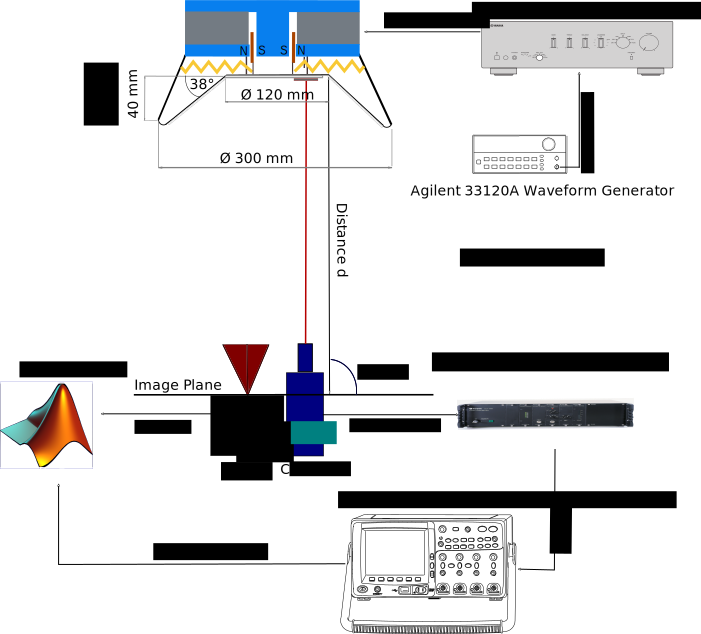
\includegraphics[width=1.0\textwidth]{Bilder/Experimental_setup_Final_1711.pdf}
	\caption{Sketch of the experimental setup}
	\label{fig:experimental_setup} 
\end{figure}     

\begin{center}
	\begin{tabular}{| l | l | l |}
		\hline
		\textbf{Device} & \textbf{Information} & \textbf{Configuration} \\ \hline
		Polytec CLV700 & HeNe Laser Safety II  & Variable laser focus   \\ \hline
		Input Module CLV-M200 & $v_{max}=1.250~mm/s$ & $2~\mu m$ Resolution  \\ \hline
		Decoder Module CLV-M030 & Resolution = $ 2~\mu m/s$ & $125~mm/s/V$  \\ \hline
		Output Module CLV-M001 & - & $5~kHz$ Low-pass filter \\ \hline
		Kinect 2 & $512x424~30$ fps & Depth resolution $1~mm$ \\ \hline
		Agilent 33120A Waveform Generator  & Uncalibrated & $0.894~V_{pp}$ \\ \hline
		Agilent DSO6054A Oscilloskop & $500~MHz$ & $1000, 500~or~250~ms~per~DIV$ \\ \hline
		Yamaha A-S500 Amplifier & $150~W$ Mono & pure direct / no filtering \\ \hline
		Matlab R2013a & - & - \\ \hline
		Subwoofer & 30'' JBL Car Tube & Paper Sticker / Reflector \\
		\hline 
	\end{tabular} \captionof{table}{Devices of experimental setup}	
\end{center}

\begin{figure}[!h]
	\centering
	\fbox{\includegraphics[width=1\textwidth]{Bilder/Versuchsaufsbau_TOF_LDV.jpg}}
	\caption{Experimental setup}
	\label{fig:ToF_LDV_Team}
\end{figure} 

\newpage
\begin{figure}[!h]
	\centering
	\fbox{\includegraphics[width=1\textwidth]{Bilder/Kinect_2_LDV_Team.jpg}}
	\caption{LDV and Kinect 2 mounted on one tripot}
	\label{fig:ToF_LDV_Team}
\end{figure} 

\begin{figure}[!h]
	\centering
	\fbox{\includegraphics[width=1\textwidth]{Bilder/Membrane_laser.jpg}}
	\caption{Membrane with white paper stickers and reflector}
	\label{fig:membrane}
\end{figure} 

\newpage

\subsection{Test Procedure}
Some fundamental boundary conditions apply for all experiments that are done. Every device should be turned on for some minutes before the execution to achieve a stable temperature. ToF cameras are in general sensitive in their accuracy for fluctuation in temperature \cite{foix2011lock}. The IR lighting and electronic heats up the device over time. The LDV is pointed together with the ToF camera on the membrane with reflector and the white paper attached to it. The membrane is in the middle of the field of view in the distance d and the viewing angle $\alpha$ to the normal vector $\vec{n}$ of plane middle surface. If no angle is given, it is kept constant at $\alpha = 0^\circ$. The LDV signal indicator should be at least at a level of about $30~\%$ to guaranty a high SNR. Afterwards, the volume of the amplifier can carefully be turned up. Ideally, no sound should be hearable with frequencies lower than $30~Hz$. In practice, the membrane creates noise in higher frequencies even if it excited in the 1 to 10 Hz range. The LDV is capable to measure this sounds as spikes on the sinus oscillation. It is a sign for an overdrive of the subwoofer. The high amplitudes can cause the membrane to detach from the tube. The attachment is checked under the highest amplitude and frequency according to equation \ref{eq:Energy_oscillation}. The tube and the structure itself should not get excited. The peak-to-peak value is displayed on the oscilloscope and should stay in a narrow band. It is an indicator for a stable oscillation at a constant amplitude \ref{chap:LDV_processing}. Every measurement point is the mean from a 4x4 pixel window that is chosen by the user as near a possible to the LDV measurement at the middle of the white paper. Since the laser reflector is also spectral reflecting the ToF IR lighting, an investigation of the same point is not possible. The reflector leads to a hole in the 3D scan. Some safety guidance for humans, environment and devices have to be kept in mind. The laser beam should never be attached in the height of the human eye to avoid damages to the retinal after long exposure. The membrane is another source of danger. High amplitudes up to $10~mm$ require the volume to be turned up to a maximum. The same volume in the audible range can damage the eardrum. So a change in frequency at the waveform generator has to be done with caution. Structures in the environment of the test are also exposed by the strong vibrations and can be excited in there eigenfrequencies. The influence of background lighting is characterized in a distance of $1.4~m$ at $3~Hz$ with $2000~W$ halogen lighting at the position of the cameras pointing on the membrane. An RGB image from the Kinect's perspective is visible in figure \ref{fig:KinectScreenshot-Color-10-58-52}\\

The data is captured in a unsynchronized way. This means, that single data points cannot be compared to each other. It is only possible to analyze single deflections to each other in the variable displacement setup. In all other configurations it is assumed, that the oscillations is kept stable over the complete acquisition time. In this way, small time delays between the ToF and LDV measurement have a small impact on the results in the frequency domain. Nevertheless a time synchronization is beneficial. Both measurements must take place in the same time span. The acquisition of both devices is started manually. At first, by the commandline on the PC to start ToF and afterwards by pressing the "Quick Print" button on the oscilloscope to acquire the LDV data. Since low frequencies can not trigger the screen, the measurement should be started when the signal trend ends at the right side of the screen.    

\subsubsection{Variable Distance}
The first parameter being changed, is the distance d of the tripot to the middle of the membrane. A high precision horizontal movement is not possible with the given equipment. The rough estimation is done with a measuring tabe. The $0^\circ$ viewing angle of the laser beam to the surface normal vector should be kept constant under all conditions. The volume and the frequency of the waveform generator $f_{ref}=3~Hz$ is unchanged for all measurement points. The  amplitude of about $4~mm$ is high enough to distinguish it from noise under the maximum distance. For every measurement point the focus of the LDV has to be readjusted to a sufficient signal level. The noise is reconsidered for every distance and can be minimized by gently moving the sensor head. The first run of the experiment is done for 3 seconds of ToF and 2 seconds of LDV. The second run will be done for 10 seconds of LDV and 8 seconds of ToF. At a distance of $1.4~m$ the setup is added with $2000~W$ of halogen lighting at the position of the camera to disturb the ToF measurement on the membrane with additional IR light.

\subsubsection{Variable Angle}   
Since there is no precise setup for the viewing angle $\alpha$ determination, it is estimated by a goniometer on the floor. In the distance of $1.4~m$ and $2.0~m$ the angle $\alpha$ is changed from $90^\circ$ to $0^\circ$ in $5^\circ$ steps at a constant frequency of $f_{ref}=3~Hz$. $\alpha$ is the angle between the optical axis of the camera and the  middle surface turning in the mathematical positive direction. The focus must be readjusted for every angle. It is ensured, that the laser points on the reflector over the complete displacement of the membrane at every angle. The area of the LDV and ToF measurement is therefore increased with higher angles. The simplest way to change the angle between the perspective and the membrane is by turning the subwoofer on the measurement point. The paper stickers are compared with each other. The one in the middle delivers a surface under the angle $\alpha$. The lower sticker has an angle of $\alpha + 38^\circ$ and the lower of $\alpha -38^\circ$ due to the cone. 

\subsubsection{Variable Frequency}
The change of frequency from $10~Hz$ to $1~Hz$ is done in a distance of $1.4~m$ at a constant volume in one $1~Hz$ steps at $\alpha = 0^\circ$ to the surface normal. Since the frequency change at the functions generator cannot be separated from a change in the maximum displacement, the amplitude cannot be kept constant for different configurations. The membrane should still be out the overdrive region to archive comparable data, at the highest frequency. The acquisition takes place at every parameter for 8 seconds to capture enough periods at the lower frequencies.     

\subsubsection{Variable Displacement}
The volume is turned up from $0~\%$ slowly for a brief moment and reduced afterwards for the investigation of different displacement of the membrane. This configuration can also be considered as an amplitude sweep, because the volume is changed during the data recording. Only a small number of oscillations is analyzed and can be compared with the idle state before and after the oscillation. The acquisition takes place for 8 second to allow enough time for turning the volume up and down manually. 

\subsubsection{Sweep}
The adjustment of the frequency versus time is called Sweep. At a constant volume, the frequency is increased manually in $0.1~Hz$ steps from $1$ to $10~Hz$. Ideally, this is done automatically by the function generator in a smaller resolution. The measurement takes place over 10 seconds with ToF and LDV. To gather all the date with the scope in this time span, $f_{sampling}$ has to be decrease to $100~Hz$. No noise should occur at the highest frequency in order to avoid deviations of the ideal sinus trend. 

\newpage

\subsection{Measurement Results}
All data is processed by the $dynKinect\_0\_3\_thesis\_evaluation.m$ Matlab script. The TimePerDIV parameter is the only number that has to be chosen manually depending on the acquisition time of the oscilloscope. From this $f_{sampling}$ results according to equation \ref{eq:scope_capture}. The wrong parameter will change the amplitudes, times and frequencies in the domains. For a comparison between the devices, raw data is transformed into the frequency domain by the fft() function shown in chapter \ref{sec:Dynamic_pixel}, \ref{chap:LDV_processing} and \ref{chap:frequency_domain}. The Short-time Fourier transform method is used for the sweep analysis. In the frequency domain, noise and dynamic are easy to separate. The strongest peak in a 4x4 pixel windows is the value that is compared and plotted versus the change of parameters. In a distance of $2.6~m$, the window still fits on the sticker of $76x39~mm$ according to equation \ref{eq:pixel_area} and figure \ref{fig:area_of_4x4_pixelwindow}. Every data point is written into a CSV file by hand. The file is shifted into the Matlab workspace afterwards. A small script called $xy\_plotter.m$ is used to plot the data into graphs automatically.

\newpage

\subsubsection{Variable Distance}

Figure \ref{fig:Distance_vs_Amp} shows the progress of a the raw and TVD filtered data versus the reference LDV measurement after 3 seconds. LDV delivers two distortions at $1.1~m$ and at $1.8~m$ that cannot be explained by the instability of the membrane. A detailed analysis in the time domain shows an error in the processing with Matlab. Plotting clarifies an unsteady trend. This behavior is not noticeable in the raw data of the oscilloscope. Equally to the $1.8~m$ position, a strong jump of about $3~mm$ can be observed in the frequency and time domain additionally. A second peak near $0~Hz$ appears in the time domain and is a measure for the offset. Such behavior cannot be observed in the ToF data. A reason for that could be noise in the LDV measurement or an incorrect integration procedure. That is why those two points are not used as a reference and not plotted in the LDV data. Apart from that, the amplitude is reconstructed with a maximum error of about $1~mm$ by ToF. The membrane works stable in a range of about $0.4~mm$ in all distances at around $3.5~mm$ amplitude according to LDV. An influence of the distance on the accuracy is not clearly visible. The TVD filter could increase the accuracy in the distance between $0.9~m$ and $1.6~m$ with fixed parameters. Strong distortions like in $1.3~m$ and $1.6~m$ are reduced. In other distances, the filtering reduces the accuracy in contrast. Figure \ref{fig:0_6m_to2_6m_3Hz_240frames} visualizes the influence of a longer acquisition time of LDV and ToF in a second series of tests. The amplitude is reconstructed by LDV in smaller range of about $0.2~mm$ with no distortions. ToF delivers a strong deviation at $0.8~m$. The reason for that could be light scattering between the sensor and the lens. Too much light is reflected from the white paper surface. Apart from that point, the amplitude is reconstructed in a band of about $0.7~mm$. In the distance of $1.3~m$ to $1.5~m$, the absolute error is minimized down to a value of $0.05~mm$. The increased acquisition time allows a better separation of the variance from the actual dynamic. Figure \ref{fig:area_of_4x4_pixelwindow} delivers the projected area of the 4x4 pixel window versus the distance at a viewing angle of $0^\circ$.

 \begin{figure}[!h]  
 	\centering
 	\includegraphics[width=0.63\textwidth]{Bilder/area_of_4x4_pixelwindow.png}
 	\caption{Theoretical area of 4x4 pixel window versus distance}
 	\label{fig:area_of_4x4_pixelwindow}
 \end{figure}        

\begin{figure}[!h]  
	\centering
	\includegraphics[width=0.95\textwidth]{Bilder/Distance_vs_Amp.png}
	\caption{Amplitude $A_p$ versus distance after 3 seconds of ToF measurement}
	\label{fig:Distance_vs_Amp}
\end{figure} 

\begin{figure}[!h]  
	\centering
	\includegraphics[width=0.95\textwidth]{Bilder/0_6m_to2_6m_3Hz_240frames.png}
	\caption{Amplitude $A_p$ versus distance after 8 seconds of ToF measurement}
	\label{fig:0_6m_to2_6m_3Hz_240frames}
\end{figure} 

A direct comparison of the time domain data of ToF in figure \ref{fig:Time_domain_ToF} and LDV in figure \ref{fig:Time_domain_LDV} shows the huge difference in the sampling rate and resolution. The digital resolution of $T_{sample} = 33.3~ms$ in time and $1~mm$ in depth is noticeable in the ToF data. Regions of high acceleration at the peaks of the displacements have sharp digital edges in the sinus trend. This leads to additional fluctuations in the peak values. The LDV data proves the high short time stability of the membrane vibration. The short spacing in time of $T_{sample} = 5~ms$ and in displacement of $2~\mu m$ very precisely reconstructs the trends. A better comparison between a set of ToF and LDV data can be done in the frequency domain after a FFT. Figure \ref{fig:Freq_domain_ToF} and \ref{fig:Freq_domain_LDV} shows the ToF and LDV in the frequency domain in $1.4~m$ distance. The difference in the amplitude $A_p$ is $0.063~mm$ and in frequency $0.117~Hz$. The obvious error in frequency can be explained by the digital resolution in time of $T_{sample}=0.033~s$. Even the first and second harmonic component are clearly defined and match to the spectrum of LDV. On other parts of the membrane, the harmonics cannot be distinguished from noise that clearly as on the oblique black cone surfaces. Figure \ref{fig:Freq_domain_ToF_2m}  and \ref{fig:Freq_domain_LDV_2m} illustrate the frequency domain in $2~m$ distance. The first and second harmonic can still be seen in the ToF spectrum. The error of the absolute peak is increased to $+0.402~mm$. In the LDV data, the third harmonic is still visible. An offset peak at $0.1953~Hz$ of $0.3618~mm$ appears in the LDV data but not in the ToF data. 

\begin{figure}[!h]  
	\centering
	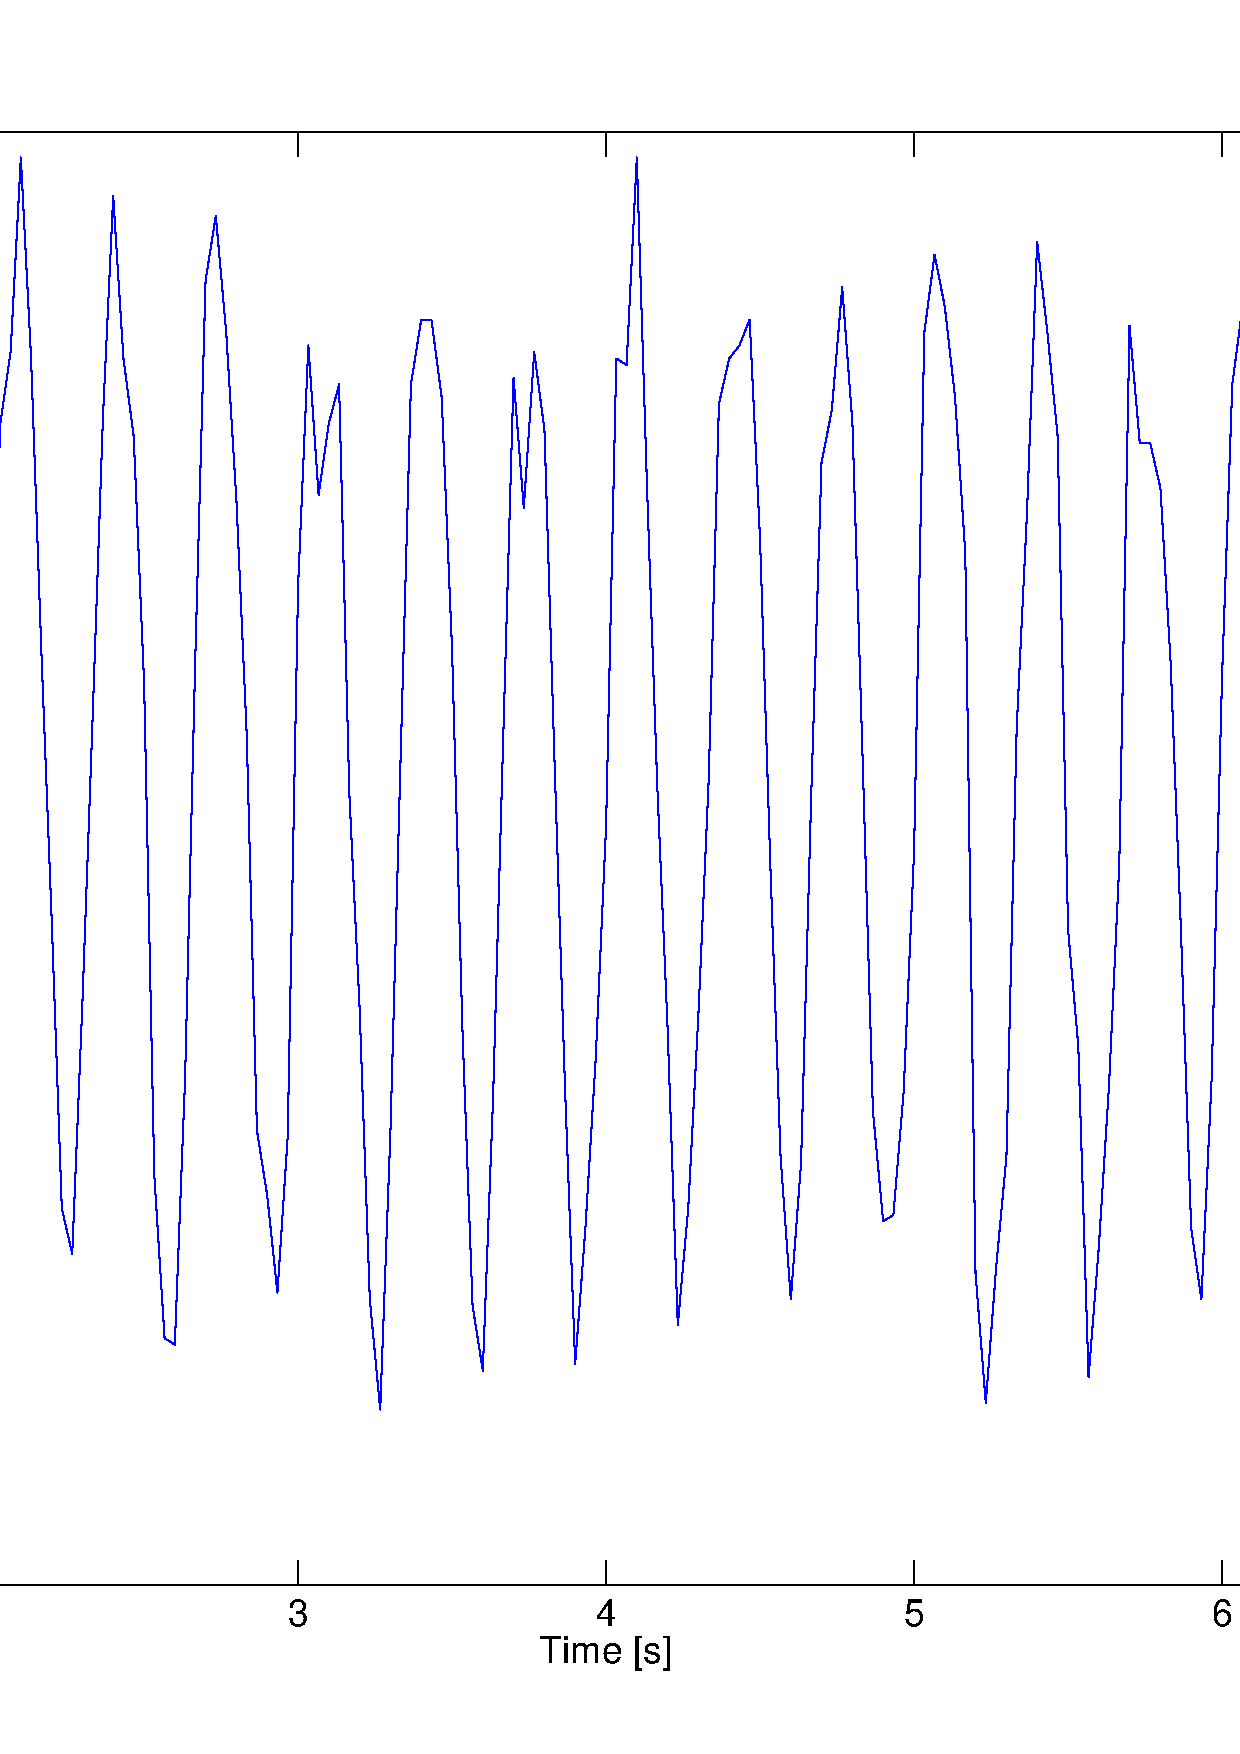
\includegraphics[width=0.80\textwidth]{Bilder/Time_domain_ToF.png}
	\caption{Time domain of ToF after $8~s$ in $1.4~m$ distance}
	\label{fig:Time_domain_ToF}
\end{figure}  

\begin{figure}[!h]  
	\centering
	\includegraphics[width=0.78\textwidth]{Bilder/Time_domain_LDV.png}
	\caption{Time domain of LDV after $8~s$ in $1.4~m$ distance}
	\label{fig:Time_domain_LDV}
\end{figure}  

\newpage
For a detailed illustration of complete surface dynamics, two new images are created from the $1.0~m$ data. Every pixel of the ToF video stream is analyzed in the FFT and a new image is plotted depending on the highest peak $A_p$ in the spectrum. Section \ref{sec:Dynamic_pixel} explains the creation of such images more detailed. The challenge is to integrate the frequency or the amplitude into a 2D plot in a huge range with a high contrast in the colorspace. The dynamic information from the video data is transferred into a single image. Figure \ref{fig:Freq_distribution} illustrates the dominating frequency distribution of $f_p$ on the membrane. Most pixels measure the correct $3~Hz$ frequency. Some areas on black oblique surfaces are dominated by noise of a random spectrum. The frequencies are shifted slightly. At the edges of the stickers, the amplitudes and frequencies are highly increased. An explanation is the a fluctuation of variance between the white and black field in the area that is observed by the pixel. The change in variance overestimates the actual defection.\
\begin{figure}[!h]
	\subfigure[ToF Frequency Domain]{\includegraphics[width=0.5\textwidth]{Bilder/Freq_domain_ToF.png}\label{fig:Freq_domain_ToF}}\hfill
	\subfigure[LDV Frequency Domain ]{\includegraphics[width=0.5\textwidth]{Bilder/Freq_domain_LDV.png}\label{fig:Freq_domain_LDV}}
	\caption{$3~Hz$ excitation in $1.4~m$ distance}
\end{figure}

\begin{figure}[!h]
	\subfigure[ToF Frequency Domain]{\includegraphics[width=0.5\textwidth]{Bilder/Freq_domain_ToF_2m.png}\label{fig:Freq_domain_ToF_2m}}\hfill
	\subfigure[LDV Frequency Domain ]{\includegraphics[width=0.5\textwidth]{Bilder/Freq_domain_LDV_2m.png}\label{fig:Freq_domain_LDV_2m}}
	\caption{$3~Hz$ excitation in $2.0~m$ distance}
\end{figure}
\newpage
 Another abnormality is given by the LDV reflector. The IR light is reflected spectral on this surface. A depth measurement is not possible here and therefore also no dynamic investigation. The static surfaces around the membrane illustrates this in chaotic colors. The dominating frequencies on the static surfaces depend on the variance that shows a very high entropy. Figure \ref{fig:Amp_distribution} clarifies the amplitude distribution. Higher values than $5~mm$ are removed to distinguish small changes in the colorspace. The white paper delivers a homogeneous variance distribution and therefore a steady amplitudes distribution. The values are underestimated or overestimated in the black oblique regions. The connection between the static and dynamic part of the membrane shows a transition of the amplitude from $4~mm$ to $0~mm$. In the upper oblique areas, the amplitude is higher than in the lower ones. An explanation for that could be the variance depending on the incident angle $\varphi$ according to equation \ref{eq:Radiance_and_Luminance_on_a_surface}. Figure \ref{fig:checkerboard} illustrates the same effect on the checkerboard. In tabel \ref{tbl:Dominating_freq_distance} and \ref{tbl:Dominating_amp_distance}, a complete overview of the distribution in frequency $f_p$ and amplitude $A_p$ is given from $0.6~m$ to $1.3~m$ for the 8 seconds measurement time. In $0.6~m$ four paper stickers cannot be analyzed. This can be explained by a saturation of the ToF Sensor by light scattering. The amount of reflected light is too high for the depth measurement. With increasing distance, the oblique black surfaces display errors in the frequency and amplitude measurement. In total, the white paper surfaces could be measured correctly in frequency and amplitude from $0.7~m$ to $2.6~m$. The amplitude distribution in $0.8~m$ shows the same error as in figure \ref{fig:0_6m_to2_6m_3Hz_240frames}. Even in a distance of $1.3~m$, the amplitude in the oblique black areas is not higher than $3~mm$ of the LDV measurement. 3D plotting of the amplitudes can help to recognize patterns in the deformations. Figure \ref{fig:Amp_distribution_3D} shows the 3D plotting by the mesh() function in Matlab of the $0.8~m$ data. Regions of different amplitude distribution can be distinguished easier. In this illustration, the sinusoidal trend of the error at the edges of the sickers becomes visible. The appearing waveform is at a constant wavelength with various amplitudes. A explanation for this behavior could be fluctuations of the variance between black and white in the pixels when the membrane is moving. To illustrate the frequency and the amplitude distribution in a single image, the frequency is plotted by mesh() and the surface color is determined by the amplitude in figure \ref{fig:_Freq_Amp_distribution_3D}. This delivers the complete dominating dynamic in a single image.\\

\begin{figure}[!h]
	\subfigure[Distribution of the $f_p$ in a distance $d=1.4~m$]{\includegraphics[width=0.5\textwidth]{Bilder/Freq_distribution.png}\label{fig:Freq_distribution}}\hfill
	\subfigure[Distribution of $A_p$ in a distance $d=1.4~m$]{\includegraphics[width=0.5\textwidth]{Bilder/Amp_distribution.png}\label{fig:Amp_distribution}}
	\centering
	\caption{Distribution of the dominating frequency $f_p$ and dominating amplitude $A_p$}
\end{figure}

Table \ref{tbl:Dominating_harmonic_distance} shows the frequency distribution $f_{ph}$ of the strongest harmonic peak. It it obvious that only the white paper surface delivers correct harmonic frequencies. In the near distance the second harmonic is stronger in some areas. The $1.2~m$ and $1.3~m$ distance delivers a more homogeneous distribution of the first harmonic. Therefore the first becomes stronger than the second harmonic. Comparing this with figure \ref{fig:0_6m_to2_6m_3Hz_240frames}, it seems that the areas where correct harmonics are indicated, is a measure for the accuracy of the complete FFT.     

\subsubsection{Variable Angle}

For the analysis of different angles to the membrane, oscillating at a constant frequency $f_{ref} = 3~Hz$ and amplifier volume, LDV is compared on the middle, lower and upper sticker with ToF. From figure \ref{fig:experimental_setup} and the photograph in figure \ref{fig:membrane} it becomes evident that the lower sticker has an viewing angle of $\alpha_l = \alpha +38^\circ$ and the upper sticker of $\alpha_u =\alpha -38^\circ$. Therefore, multiple parameters can be investigated in a single image. The reference measurement with LDV shows a trend that fits to the expected values given by the physical model in section \ref{sec:bias_membrane} for the $1.4~m$ and $2.0~m$ distance. The amplitude $A_p$ decreases with the cousins of the angle $\alpha$. The ToF results on the lower sticker can follow the trend of LDV with a small offset of about $-0.2~mm$ up to $20^\circ$ in both distances. From $35^\circ$ to $45^\circ$ this gets even smaller. This effect can be explained by the reduction of the normal angle to the image sensor with higher angles up to $38^\circ$. The middle and upper sticker delivers an overestimating of the amplitude with increasing angle. The sequence of images in table \ref{tbl:Dominating_amp_angle} shows regions of high amplitudes up to $10~mm$ on the sicker. The inhomogeneous distribution between single pixels is reduced by the 4x4 pixel windows. It is used to plot the results from figure \ref{fig:Amplitude_vs_angle_1_4m} and \ref{fig:Amplitude_vs_angle_2m}. In the $2~m$ distance, the trend is similar up to $20^\circ$. The middle sticker loses the correct frequency measurement at $30^\circ$. Noise overlies the actual dynamic of the membrane. The middle surface however still delivers the correct frequency with amplitude beneath the LDV values up to an angle of $25^\circ$. This fits to the physical model. At viewing angles $\alpha>25^\circ$, the size of the pixels play an additional role. Various distances are measured inside one pixel. The area observed in the window increases. Therefore, the model does not apply anymore. Another problem is that the analysis of the high angles is done on a inhomogeneous distributions. The value strongly depends on the position where the window was placed by the user. Tabel \ref{tbl:Dominating_freq_angle} delivers a detailed overview on the regions that can be investigated in frequency and therefore in amplitude. The black mat region around the sticker in the middle of the membrane provides the right frequency in all distances from $0^\circ$ to $45^\circ$. Only the upper sticker shows variation in the frequency on single pixel under high angles in the long distance. 

\begin{figure}[!h]  
	\centering
	\includegraphics[width=0.8\textwidth]{Bilder/Amp_vs_angle_1_4m_new_alpha.png}
	\caption{Dominating amplitude $A_p$ under variable angle in $1.4~m$}
	\label{fig:Amplitude_vs_angle_1_4m}
\end{figure}

\begin{figure}[!h]  
	\centering
	\includegraphics[width=0.8\textwidth]{Bilder/Amp_vs_angle_2m_new_alpha.png}
	\caption{Dominating amplitude $A_p$ under variable angle in $2~m$}
	\label{fig:Amplitude_vs_angle_2m}
\end{figure}

\subsubsection{Variable Frequency}

The measurement of different steady frequencies at a constant volume over a time span of $3~s$ is plotted in figure \ref{fig:1_to_10Hz} and figure \ref{fig:1to10Hz_Frequency_Plot}. The measurement at a frequency of $4~Hz$ shows the strongest variation in the amplitude $A_p$ of about $1.4~mm$. At $2~Hz$, the strongest peak in the amplitude is recognizable with $6.6~mm$ ToF and $5.6~mm$ LDV. This behavior matches the observations by sight. After that, the amplitude decreases steadily down to $3.7~mm$ at $10~Hz$. The error in the amplitude is also reduced with higher amplitudes. This matches the results from figure \ref{fig:0_6m_to2_6m_3Hz_240frames}. More periods are acquired in the $3~s$ at higher frequencies. Therefore, the actual amplitude can be estimated better. The frequency measurement matches between LDV, ToF and the Waveform Generator for every data point. ToF has an error in the period smaller than $T_{sample}=0.033~s$. A connection between the error and the frequency is not visible on the white markers. The frequency distribution in table \ref{tbl:Dominating_freq_vs_freq} contrary, shows more errors on the black oblique surface with higher oscillating frequency.

\begin{figure}[!h] 
	\centering
	\includegraphics[width=0.8\textwidth]{Bilder/1_to_10Hz_amp.png}
	\caption{Amplitude $A_p$ versus different oscillation frequencies $f_{ref}$ of the membrane}
	\label{fig:1_to_10Hz}
\end{figure}

\begin{figure}[!h]  
	\centering
	\includegraphics[width=0.8\textwidth]{Bilder/1_to_10Hz.png}
	\caption{Frequency $f_p$ versus different oscillation frequencies $f_{ref}$ of the membrane}
	\label{fig:1to10Hz_Frequency_Plot}
\end{figure}

\newpage
\subsubsection{Variable Displacement}

The analysis of the variable displacement offers the opportunity to directly compare deflections on the time axis. Ideally, the samples should be phase synchronized for a direct comparison, but since both measurement are running in free-run mode, this is not possible. Figure \ref{fig:Variable_displacement_ToF} shows the ToF data in a time window of 5 seconds. At the beginning and the end of the signal where no deflection appears, the noise is visible. In the LDV data, plotted in figure \ref{fig:Variable_displacement_LDV}, the variance in the measurement is not recognizable at the start and end of the signal. The signal course shows a sinusoidal trend without any abnormality. The deflection in the positive direction seems to be minimal higher than in the negative direction. In both signals, the 12 deflections can be identified and assigned. The low sampling rate of the ToF measurement causes a mismatch in the amplitudes. To compensate the difference in the offset between both signals the peak-to-peak $A_{pp}$ amplitudes are plotted against each other for every deflection in figure \ref{fig:displacement_comparision}. ToF shows an overestimating between $1$ and $2~mm$ until deflection 9, that can be explained by the high variance of ToF. Subsequently, the ToF data underestimates the true LDV data. This point of change is the same deflection where both $A_{pp}$ values are decreasing. In figure \ref{fig:Time_domain_Sweep_ToF} and figure \ref{fig:Time_domain_Sweep_LDV}, the frequency domain is plotted. ToF overestimates the amplitude by $1.428~mm$. The first and second harmonic can still be found in the ToF spectrum. Also, the offset peak is visible in both data.
 
\begin{figure}[!h]  
	\centering
	\includegraphics[width=0.9\textwidth]{Bilder/PP_comparison.png}
	\caption{Direct deflection comparison in peak-to-peak $A_{pp}$ value. }
	\label{fig:displacement_comparision}
\end{figure}

\newpage

\begin{figure}[!h]  
	\centering
	\includegraphics[width=0.8\textwidth]{Bilder/Variable_displacement_LDV.png}
	\caption{Variable displacement of the LDV data $1.4~m$ distance}
	\label{fig:Variable_displacement_LDV}
\end{figure}



\begin{figure}[!h]  
	\centering
	\includegraphics[width=0.8\textwidth]{Bilder/Variable_displacement_ToF.png}
	\caption{Variable displacement of the ToF data in $1.4~m$ distance}
	\label{fig:Variable_displacement_ToF}
\end{figure}

\begin{figure}[!h]
	\subfigure[Frequency domain of ToF data]{\includegraphics[width=0.5\textwidth]{Bilder/FFT_variable_displacement.png}\label{fig:FFT_variable_displacement}}\hfill
	\subfigure[Frequency domain of LDV data]{\includegraphics[width=0.5\textwidth]{Bilder/FFT_variable_displacement_LDV.png}\label{fig:FFT_variable_displacement_LDV}}
	\centering
	\caption{ToF and LDV comparision of $3~Hz$ oscillation in $1.4~m$ distance}
\end{figure}
\newpage 

\subsubsection{Sweep}
The sweep is a simple way to analyze multiple frequencies in a single measurement in order to derive the behavior of a system in a broad band. Figure \ref{fig:Time_domain_Sweep_ToF} plots the Time domain of the sweep from $1~Hz$ to $10~Hz$. The offset of the sinus trend is constant over the complete time. The quantization error and the variance cause a fluctuation in the amplitude. The LDV data, in contrast, has an offset that is unsteady over time. A reason could be a numerical integration error or noise that was not properly filtered by a high-pass filter before the analysis.  


\begin{figure}[!h]  
	\centering
	\includegraphics[width=0.8\textwidth]{Bilder/Sweep_Time_domain_ToF.png}
	\caption{$1~Hz$ to $10~Hz$ sweep in $1.4~m$ distance captured with ToF}
	\label{fig:Time_domain_Sweep_ToF}
\end{figure}

\begin{figure}[!h]  
	\centering
	\includegraphics[width=0.9\textwidth]{Bilder/Sweep_Time_domain_LDV.png}
	\caption{$1~Hz$ to $10~Hz$ sweep in $1.4~m$ distance captured with LDV}
	\label{fig:Time_domain_Sweep_LDV}
\end{figure}

\newpage
Since a sweep contains all frequencies in the spectrum, the standard Fourier transform of the complete signal shows superimpositions between the single peaks. An analysis for separated frequencies is not possible. For that reason, the signal is analyzed by the Short-time Fourier transform and plotted in a spectrogram. The 10 seconds of measurement time are separated into 9 slots for the frequencies of $1~Hz$ to $10~Hz$. This is done by a fixed number of samples for the processing represented by NFFT of 128 for LDV and 32 for ToF. A hanning window is used to reduce the influence at the window edges. Figure \ref{fig:spectogram_Variable_displacement_ToF} represents the spectrogram of the ToF data. Every step from $1~Hz$ to $10~Hz$ is visible without any offset. The $1~Hz$ range indicates a reduced amplitude that is also visible in the time domain. Afterwards the amplitudes stay stable at about $45~dB$. Harmonic frequencies can be identified for some ranges with amplitudes of about 15 dB. 

\begin{figure}[!h]  
	\centering
	\includegraphics[width=0.9\textwidth]{Bilder/ToF_Freq_vs_Time.png}
	\caption{Spectrogram of the sweep ToF data in $1.4~m$ distance}
	\label{fig:spectogram_Variable_displacement_ToF} 
\end{figure}

Figure \ref{fig:spectogram_Variable_displacement_LDV} shows the same sweep measured by LDV. In contrast to ToF, an offset of the signal appears at $1~Hz$, $2~Hz$ , $3~Hz$ , $7~Hz$ and $9~Hz$ that is also visible in the time domain. Apart from that, every frequency is identified. The different between the amplitudes is caused by a number of samples that are processed. Due to the low variance and high resolution of LDV, the first, second and third harmonic for every frequency are represented in the spectrogram. 

\begin{figure}[!h]  
	\centering
	\includegraphics[width=0.9\textwidth]{Bilder/LDV_Freq_vs_Time.png}
	\caption{Spectrogram of the sweep LDV Data in $1.4~m$ distance}
	\label{fig:spectogram_Variable_displacement_LDV}
\end{figure}  
 
\newpage
\subsubsection{Influence of Background Lighting on Dynamic Measurement}
For estimating the influence of the $2~kW$ halogen lighting, which is also done for the static in section \ref{chap:static_Lighting}, the distribution of the harmonics will be used as an indicator for the quality of the measurement. Figure \ref{fig:harmonics_dark} clarifies the distribution of the harmonics of a $3~Hz$ oscillation in $1.4~m$ distance under ideal dark conditions. The white paper surface delivers the first and the second harmonic. Figure \ref{fig:harmonics_haloge}, in contrast, shows the impact of $2000~W$ halogen lighting. The harmonics are overlaid by the increase of the variance.  

\begin{figure}[!h]
	\subfigure[Frequency Distribution of the dominating harmonic peaks $f_{hp}$ at darkness]{\includegraphics[width=0.47\textwidth]{Bilder/harmonics_dark.png}\label{fig:harmonics_dark}}\hfill
	\subfigure[Frequency Distribution of the dominating harmonic peaks $f_{hp}$ at $2~kW$ halogen lighting]{\includegraphics[width=0.47\textwidth]{Bilder/harmonics_halogen.png}\label{fig:harmonics_haloge}}
	\centering
	\caption{Harmonic frequency distribution $f_{hp}$}
\end{figure}
\newpage

Looking at the frequency distribution in figure \ref{fig:Frequency_Distribution_lighting}
of the dominating peak shows that especially on the black oblique the frequency is not estimated correctly. The influence is explicit in the left lower corner. A spread reflection from the halogen lighting directly points into the camera.

\begin{figure}[!h]
	\subfigure[Frequency Distribution of the dominating peaks $f_p$ at darkness]{\includegraphics[width=0.47\textwidth]{Bilder/dominating_frequency_darkness.png}\label{fig:dominating_frequency_darkness}}\hfill
	\subfigure[Frequency Distribution of the dominating peaks $f_p$ at $2000~W$ halogen lighting]{\includegraphics[width=0.47\textwidth]{Bilder/dominating_frequency_halogen.png}\label{fig:dominating_frequency_halogen}}
	\centering
	\caption{Dominating frequency distribution $f_p$}
	\label{fig:Frequency_Distribution_lighting}
\end{figure}

From the amplitude distribution represented in figure \ref{fig:Amplitude_Distribution_lighting} it becomes obvious, that the markers are influenced less than the black oblique region. The dynamic of the static part around the membrane also increases in its amplitude. The results match to the static investigation that has been done. The high amount of IR lighting disturbs the dynamic measurement. The noise level is increased and superimposes the measurement of the dynamic. 

\begin{figure}[!h]
	\subfigure[Amplitude distribution of the dominating harmonic peaks $A_{p}$ at darkness]{\includegraphics[width=0.47\textwidth]{Bilder/dominating_amplitude_darkness.png}\label{fig:dominating_amplitude_darkness}}\hfill
	\subfigure[Amplitude distribution of the dominating harmonic peaks $A_{p}$ at $2~kW$ halogen lighting]{\includegraphics[width=0.47\textwidth]{Bilder/dominating_amplitude_halogen.png}\label{fig:dominating_amplitude_halogen}}
	\centering
	\caption{Amplitude distribution $A_p$}
	\label{fig:Amplitude_Distribution_lighting}
\end{figure}



\newpage
\subsection{Conclusion}
Even if the experimental setup and analysis does not correspond to all scientific standards, the overall result can be used to get an wide overview on the dynamic behavior of ToF in comparison to LDV. The variable distance setup shows errors in the LDV and ToF measurement, caused by systematic errors like range distortion or non systematic errors like light scattering. The unsteady membrane vibration additionally influences the interpretation of the data. A total fluctuation of $4~mm$ in the amplitude is recognizable in the reference LDV data of the variable distance. Electrical noise in the experimental setup and the quality of the membrane itself could be a reason for that behavior. The fact that the Kinect 2 functionality and configuration is not completely open is another challenge in the analysis. The detailed preprocessing of the images inside the camera is still unknown. Nevertheless, the device is able to measure the dynamic of an oscillating system starting at an amplitude of $1~mm$ up to a frequency of $10~Hz$. The distance of about $1.4~m$ to the camera provides the smallest error of $0.05~mm$ at a measurement time of $8~s$ and amplitude of $4~mm$. In theory, a measurement up to $15~Hz$ is possible by the Nyquist Shannon sampling theorem. The ToF data delivers the correct frequency under high viewing angles $\alpha$ up to $45^\circ$ on highly diffuse reflecting surfaces like paper in the middle of the membrane. The amplitudes are overestimated with increasing viewing angles. In contrast, LDV shows an underestimating of the amplitude $A_{p}$ with higher viewing angle. The speed vector in the direction of the laser decreases. The sweep analysis indicates that even amplitude and frequency are reconstructed in very short time spans of about $1~s$ from $1~Hz$ to $10~Hz$. It was possible to synchronize a point in time of two measurements with the variable displacement function. Unsteady processes could be compared in both data sets without a precise synchronization of the LDV sampling rate and exposure time of the ToF camera. A direct comparison between single displacements showed a maximal difference of $2~mm$ in the peak-to-peak value $A_{pp}$. The measurement of the $3~Hz$ oscillation confirms this result. The amplitudes $A_p$ are estimated from $0.6~m$ to $2.6~m$ with a maximum difference of $1~mm$. Even the first and second harmonic are reconstructed on the white paper surface. The distribution of the harmonics is an indicator for the accuracy of the measurement. The influence of background IR lighting shows a strong impact on the black oblique surface. The vibration dynamics disappear in the noise floor. The dominating frequency is still identifiable, but the second harmonic disappears on the white paper surfaces. In general, most hypotheses could be proven with a small exception. The advantages of the TVD filter is not clearly visible in the variable distance measurement. A reason for that could be processing of the raw data with the wrong parameters. Intensity images and the ToF phase shift are necessary to apply the filter in the correct manner.\\  

Dynamic investigations with ToF deliver a high improvements compared to other methods like strain gauge, stereo triangulation or LDV. Complete surfaces can be investigated fast and in parallel without a direct contact to the test body. Only a highly diffuse reflectance surface under a low viewing angle $\alpha<45^\circ$ must be guaranteed for a high signal-to-noise ratio. Apart from that, the Kinect 2 delivers a precise low cost device for dynamic investigations. The images can easily be processed with Matlab. A complex calibration is not necessary. The frequency and amplitude distribution delivers a high validation of a surface dynamic.

\section{Outlook}
\subsection{Advancements in the Experimental Setup and Analysis}
A scientific or industrial rated ToF camera is indispensable for future precise analysis for deformation measurement. A real raw data access is necessary for a widespread post-processing. Low level access for configurations like the IR modulation frequency $f_{mod}$ or the integration time $\Delta t$ are vital for adjusting the camera to different applications. A hardware trigger input enables a precise synchronization between LDV and ToF. Therefore, individual measurement samples can been compared between both data sets. An exchangeable lens is also an important advantage. The field of view can be adjusted to the region of interest. This also requires a modification of the illumination to the new field of view. The odos real.iZ-1K ToF camera, visible in figure \ref{fig:odos_real_iK_1K}, fulfills all these requirements with the highest number of pixels that can actually be found on the market. The high speed of $100~fps$ enables the investigation of an ordinary membrane up to $50~Hz$. Therefore, the range of most common structural vibrations is covered.\\

As test body the subwoofer membrane is not the ideally device. A professional shaker for structural investigations would be a better solutions, because frequency and amplitude can be adjusted precisely and held constant over time. The configured parameters deliver an additional reference to the LDV measurement. The superimposing of multiple vibrations enables the investigation of complex excitations between different sources. A high-end subwoofer in a high noise free experimental setup at audible operations frequency could also deliver a more stable behavior. With higher frame rates of the camera the membrane can be investigated in the designed operation range.\\

For a more precisely acquisition of the LDV data, an oscilloscope with a higher data storage capability is necessary. Consequently, the data can be captured with a higher sampling rate over a longer timespan. With frequencies above $10~Hz$, the trigger mode can be used for an automatic acquisition of the data. Additional investigations in the LDV measurement is necessary. The reason why some data is lost is still unknown. A low pass filter for the filtering of the offset should deliver a signal that can be compared better to the ToF data.\\ 

One strong error source in the experimental setup is the user defined measurement window with the mouse cursor. Since the white marker delivers a clear boarder to the black background, it should be possible to automatically detect the position and angle of the windows in every image. Position and number of pixels that are averaged can be fitted to the size of the marker. The existence of the harmonic frequencies in the spectrum could additionally be used to filter pixels with a low SNR out of the measurement window. The distribution of the harmonic peaks shows, that regions with a high SNR correspond to regions with a high reflectivity and therefore to higher accuracy. The distribution of the harmonics depending on the viewing angle is another investigations that delivers more information on this experimental setup.\\

The creation of the frequency and amplitude distribution images offers improvements: The images could be filtered by a proper TVD or a common image filter to improve the validity. Other algorithms for the filtering of the images or the resulting depth could also help to increase the quality of the data.\\  

A direct interface between the camera and the software is desirable for dealing with Kinect 2 inside of Matlab. Therefore, a direct live processing of the data is possible. This should simplify the scientific work with the camera remarkably. With the near-field firmware update, the range is reduced from $10~cm$ to $1~m$ \cite{nearfieldKinect}. This option is also very interesting for the deformation measurement. Since the accuracy of ToF decreases with the distance, areas can be analyzed with a very high depth accuracy at a high number of pixels. The RGB images of the camera in combination with the ToF images deliver another way for increasing the depth accuracy. Therefore, a combination between stereo triangulation and ToF is possible \cite{dal2010probabilistic}.    
\newpage

\subsection{Static Calibration and Angle Calculation}
The static calibration of a ToF system is an important step that has to be done before further dynamic investigations. In this thesis this was only possible by some rough estimations in a rough experimental setup. The influence of different surfaces, geometries and perspective delivers the base for the dynamic investigation. When a geometry cannot be measured in the static range, a dynamic investigation is not possible. The checkerboard with different colors and surface materials could be a first step. With a complex system like odos real.iZ-1K, it is anyways necessary to calibrate the camera, since depth data depends on the field of view and other configurations. A calibration of the Kinect 2 was not necessary, because the camera is already calibrated by Microsoft to a fixed configuration.\\ 

The influence of the variance versus the angle to the surface normal vector is an important investigation which is missing in this thesis. Only with this data, the dynamic behavior can be fully interpreted. An automatic calculation of the normal surface vector to the optical axis is possible with the gradient function presented in equation \ref{eq:grad}. Therefore it enables to calculate the angle of the investigated window and the error that results out of this.

\subsection{Applications in Structure and Machine Observation}
In the next step, the vibration investigations with ToF should be enlarged to a real engine or a dynamic structure like a aircraft wing. With vibration amplitudes higher than $1~mm$, the Rotax 912 ULS in the propulsion laboratory of the University of Applied Science Aachen should deliver an ideal test body. The vibrations under different frequencies in multiple directions on a complex surface represents a challenge in the experimental setup and analysis. The observation of machines could be a large application field for ToF. Disturbances in the operation are often indicated by a change in the dynamic behavior. This does also apply to structures like bridges or buildings. A change of the dynamic behavior could be a indicator for a weakening of the structure. 
 
The analysis of an aircraft wing should deliver detailed data of the aerodynamic effects like flatter and other aerodynamic load under different flight conditions. The landing phase is the most interesting situation for an deformation analysis, because most structural damages emerge here. A high resolution, high depth accuracy, long range and high speed ToF measurement should deliver all deformation of the outer geometry. The determination of flight control surfaces in 3D and the resulting angles and deformations delivers detailed information on the aerodynamic behavior.

\newpage

\subsection{Dynamic Investigations of Rotating Parts}
The trend to high speed ToF cameras with very short integration times could soon enable the recording of fast rotating parts like turbines or compressors. Polytec announced with the epc660 ToF image sensor a device, that allows up to $4000~fps$ at 160x30 pixel. In this way the movement of the blades is recorded multiple times per rotation in 3D. Geometries and deformations of the surfaces are acquired contact-less and parallel. For a detailed investigation of the rotation, a synchronization between the camera and the rotor is necessary to captured the 3D at defined positions. A laser barrier or another optical trigger can deliver a very precise and fast trigger for the camera setup.\\

One major problem that will occur is motion blur that depends on the integration time. Equation \ref{eq:motion_blur} delivers the connection between the exposure time, comparable to the integration time, and the motion blur that occurs. Assuming a blade tip speed of the $340~m/s$ and a allowed motion blur of $0.1~mm$ the integration time needs to be $0.29~\mu s$. A very strong ToF light source will be necessary to create sufficient light for a high SNR ratio leading to a proper 3D scan.

\subsection{Application in Aerodynamic and Structural Test Facilities}
Test facilities for aerodynamic and structural investigations have a high need for a detailed investigation of the surface dynamic and geometry. Since ToF cameras works with no forcing need of markers, static and dynamic investigation are possible with a single device from one point of view. Without the disturbing markers, the boundary layers is not influence anymore. The small size and construction without any mechanical parts enables various integration possibilities. From the 3D data multiple informations like angles, distances or dynamics can be captured from a single measurement.\\ 

The 3D data can additionally be used to integrate other measurements devices into a common point cloud. Therefore a ToF camera enables the integration of different optical measurement systems like Particle Image Velocimetry (PIV) or Pressure Sensitive Paint (PSP) into a common 3D mesh. With a proper synchronization between all devices the integration of all optical measurement data into one time line is possible. In such an experimental setup the deformation, aerodynamic boundary layer and vortexes can be compared to each other. The ToF data delivers in real time all geometries and dynamics, which are necessary to integrate the other measurements. The field of view, viewing angle and position of every camera must be calibrated for this setup. Figure \ref{fig:PIV_fig2a_xl.jpg} illustrates a combination between PIV and PSP for aerodynamic investigations on a delta wing. The angular velocity $\omega$ is given in the planes of the PIV measurement. PSP delivers the pressure distribution of the complete surface.  With a additional ToF measurement all deformations, angles of control surface and geometries are integrated. This allows the connection between surface dynamic and aerodynamic.
\medskip

\begin{figure}[!h]  
	\centering
	\includegraphics[width=0.7\textwidth]{Bilder/PIV_fig2a_xl.jpg}
	\caption{PIV and PSP on a delta wing \tiny DLR
		Institute of Aerodynamics and Flow Technology 2014}
	\label{fig:PIV_fig2a_xl.jpg}
\end{figure}  
